\chapter{Anhang} \section{Anleitungen zur Justage der \( \upmu \)PL}\label{Justage}
Da der Aufbau der \( \upmu \)PL im Rahmen dieser Masterthesis stark verändert wurde,
soll im Folgenden die Justage beschrieben werden. \begin{itemize} \item Laser
einschalten \item Strahl mit \textbf{M1} durch Pinhole \textbf{P1} fokussieren,
auf freien Strahlengang achten \item Mit \textbf{M3} auf Target \textbf{T2} an
Beamdump \textbf{D2} zentrieren \item Prisma verdrehen (NUR HINTERE SCHRAUBEN,
NICHT SEITLICH) um durch Pinhole \textbf{P2} zu kommen \item Beamwalk: Spiegel
\textbf{M3} und Prisma abwechselnd verdrehen: Mit Spiegel auf \textbf{P2}
zielen, mit Prisma auf Target \textbf{T2}, danach \textbf{P2} schließen. Für die
Optimierung der Ausgangsintensität empfiehlt sich  beim Zielen auf \textbf{P2}
die Leistungsdiode zu benutzen. \item Aufweitungslinse \textbf{L1} einsetzen und
auf Target \textbf{T2} zielen \item Hilfsspiegel \textbf{M7} einbauen, Spiegel
\textbf{M5} hochklappen. \item Beamsplitter \textbf{BS3} so einstellen, dass
Strahl durch die Rückseite des Schraubtargets \textbf{T3} im Objektivhalter
fällt. \item Gegebenenfalls die Weißlichtausleuchtung mit Spiegel \textbf{M6}
wiederherstellen, Laser danach mit \textbf{M5} zurück auf Target \textbf{T3}
zentrieren  \item Mit Hilfspiegel \textbf{M5} wieder durch die Vorderseite von
\textbf{T3} auf Schraubtarget \textbf{T4} im Filterrad \textbf{W} zielen. \item
Beamwalk: Mit Hilfsspiegel \textbf{M5} auf Target \textbf{T4} zielen, mit
Beamsplitter \textbf{B3} auf die Vorderseite von Target \textbf{T2}, bis der
Strahl mittig die beiden Targets trifft. Gegebenenfalls Strahl während des
Beamwalks mit \textbf{M5} nachjustieren. \item Klappspiegel \textbf{M8}
hochklappen, Filterrad \textbf{W} auf leer drehen, Schraubtarget \textbf{T4}
entfernen und auf Target \textbf{T5} fokussieren \item \textbf{M8}
herunterklappen und mit Spiegel \textbf{M9} auf Schraubtarget \textbf{T6} am
Monochromatoreingang fokussieren \item Schraubtarget \textbf{T3} entfernen und
Tubus mit Spiegel in den Objektivhalter schrauben, diesen verdrehen, um auf
\textbf{T6} zu zielen \item Shutter schließen, passendes Objektiv einschrauben,
Hilfsspiegel \textbf{M7} entfernen, Probe an der Stage montieren und Stage
einsetzen \item Weißlichtquelle anschalten, Proben grob fokussieren, dann auf
Monitor scharf stellen (durch Entfernung Objektiv-\textbf{PS-$\upmu$}) \item
Optische Dichte \textbf{OD} 5-6 einstellen, Shutter auf, um Laserspot auf
Monitor zu sehen \item Prisma und Stellschrauben der Aufweitungslinse
\textbf{L1} verdrehen bis ein schöner elliptischer Spot zu sehen ist \item 355
nm-Filter an Filterrad eindrehen \end{itemize} \begin{figure}[h] \centering
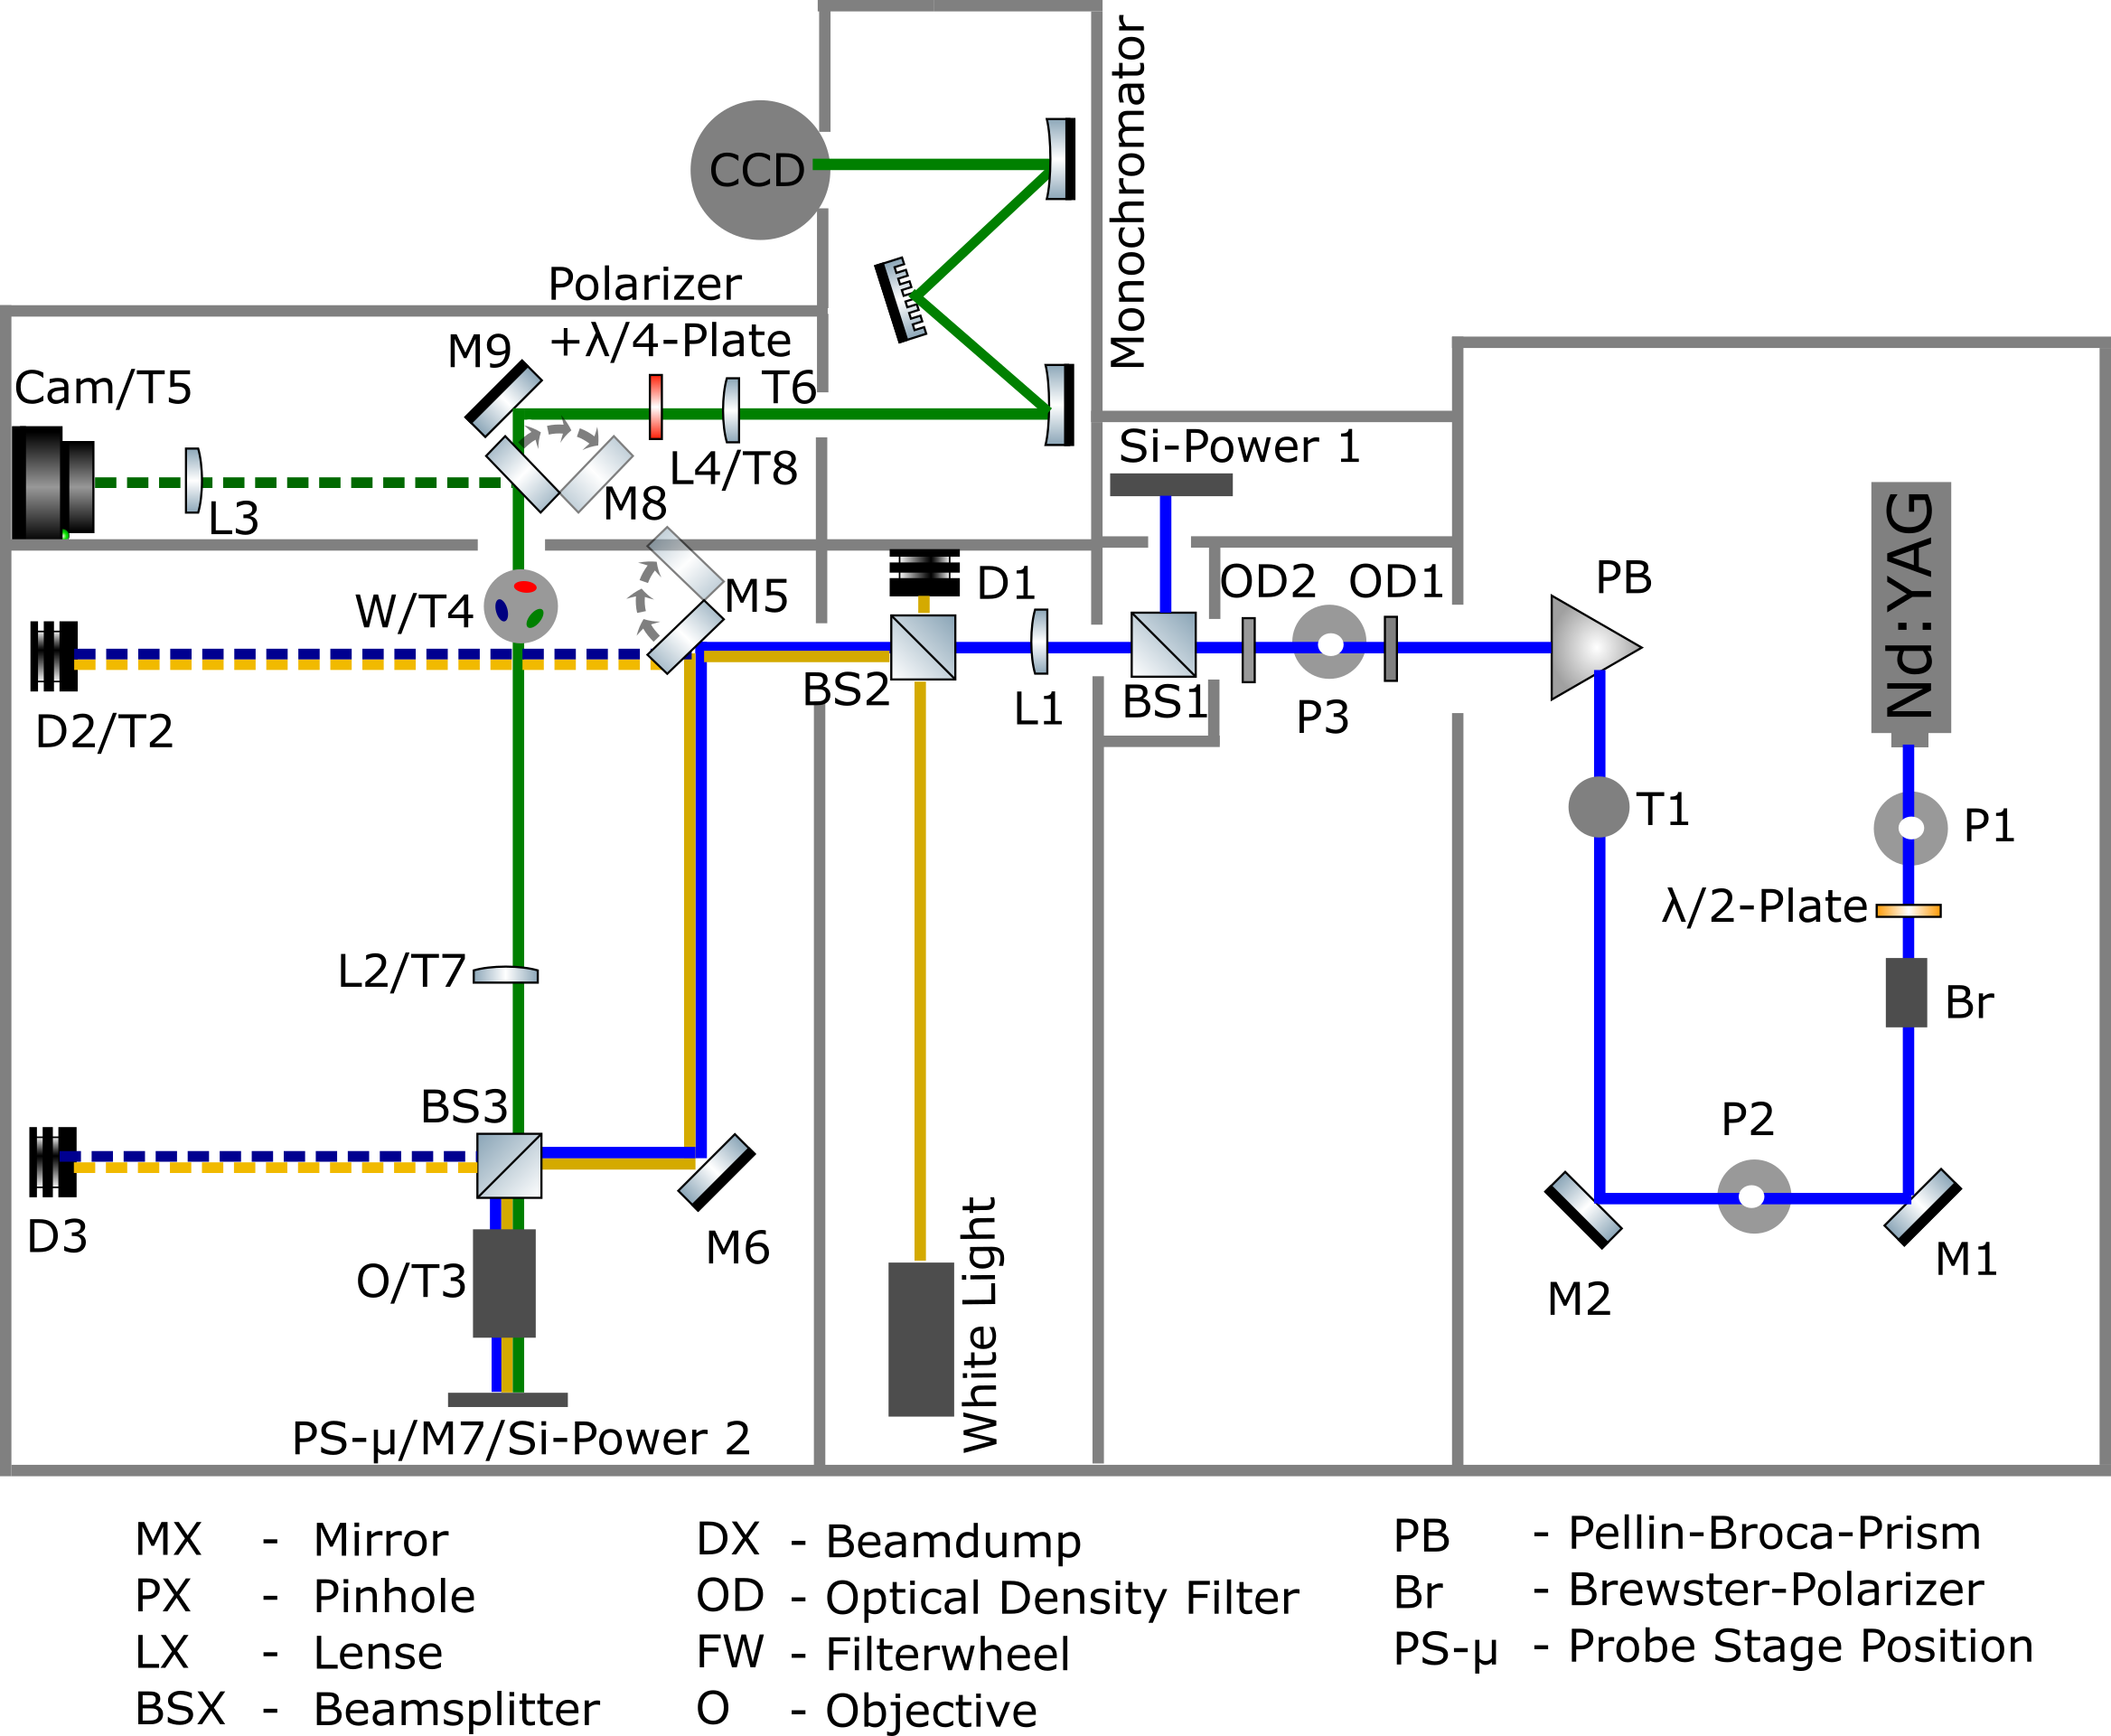
\includegraphics[width=0.75\textwidth]{Bilder/Anhang/justage} \caption[Justage
$\upmu$-PL]{Aufbau der $\upmu$-PL mit ComponentLibrary\cite{lib}.} \end{figure}
\label{JustImg} \newpage \section{Leistungsmessung} \label{Leistmess} Für
Intensitätsvariationen über mehrere Größenordnungen ist es wichtig zu wissen,
wie sich das optische System verhält, um ggf. Nichtlinearitäten zu
berücksichtigen. Dies wurde im Folgenden analysiert. \begin{figure}[b]
\centering 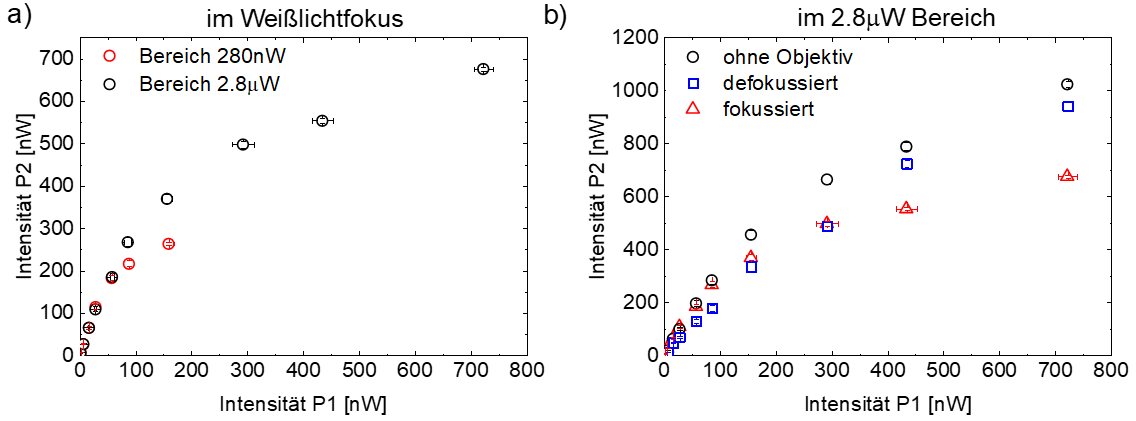
\includegraphics[width=1\textwidth]{Bilder/Anhang/Bereichsvergleich}
\caption[Vergleich Leistungsmessung]{Vergleich der Leistungsmessung a) der
unterschiedlichen Messbereiche der Leistungsmessungsdiode am Probenort im
Weißlichtfokus (P2) mit der Intensität hinter dem Filterrad (P1) b) am Probenort
(P2) im und außerhalb des Weißlichtfokus sowie ohne Objektiv.} \label{P1P2}
\end{figure} Hierzu wurde die Intensität an Si-Power 2 (P2) über der Intensität
des Lasers an Si-Power 1 (P1) (s.\autoref{JustImg}) aufgetragen. In
\autoref{P1P2} a) wurde die Messdiode in den Weißlichtfokus des Objektivs
gerückt, sodass der Laserspot ungefähr die Ausdehnung besitzt, mit der in den
Experimenten gearbeitet wird. Hierbei wurden zwei Messbereiche (bis 280 nW und
bis 2.8 $\upmu$m) der Diode verglichen. Es zeigt sich, dass beide Messbereiche
bis 80 nW identische Ergebnisse erzielen, es aber ab 100 nW zu deutlichen
Abweichungen zwischen den beiden Messbereichen kommt. Aus der Messung von
\autoref{P1P2} b)) geht hervor, dass die Messdiode im Weißlichtfokus schnell
absättigt. Die Ursache hierfür liegt in der Funktionsweise der Diode begründet.
Sie ist für Dauerstrichlaser (engl. \textit{continous wave}, kurz \textit{cw})
ausgelegt. Der Messbereich bis 280 nW schneidet also die Intensitätsspitzen des
gepulsten Nd:YAG-Lasers über 280 nW ab. Da im zeitlichen Mittel aber die
Intensität unter den 280 nW liegt, erkennt die Software im automatischen Betrieb
nicht, dass sie in den nächst höheren Bereich hätte wechseln müssen. Dies führt
zu einer Sättigung. Es ist also ratsam die Intensität außerhalb des
Weißlichtfokus zu messen. Zudem sollte für alle Intensitätsmessungen (auch an
Si-Power 1) für Messungen größer 100 nW der Bereich bis 2.8 $\upmu$W verwendet
werden. \section{Herleitung Korrektur der Abbildung} \label{correct} Projiziert
man eine Kugelfläche auf einen ebenen Detektor, wie beim Fourierimaging der
Fall, so kommt es für höhere Raumwinkel zu Verzerrungen sowohl in der Skalierung
als auch in den Intensitätsdichten. Diese Fehler lassen sich durch eine
Transformation der Koordinatensysteme beheben. Dies soll im Folgenden
ausführlich hergeleitet werden. \\ \\ \begin{figure}[h] \centering
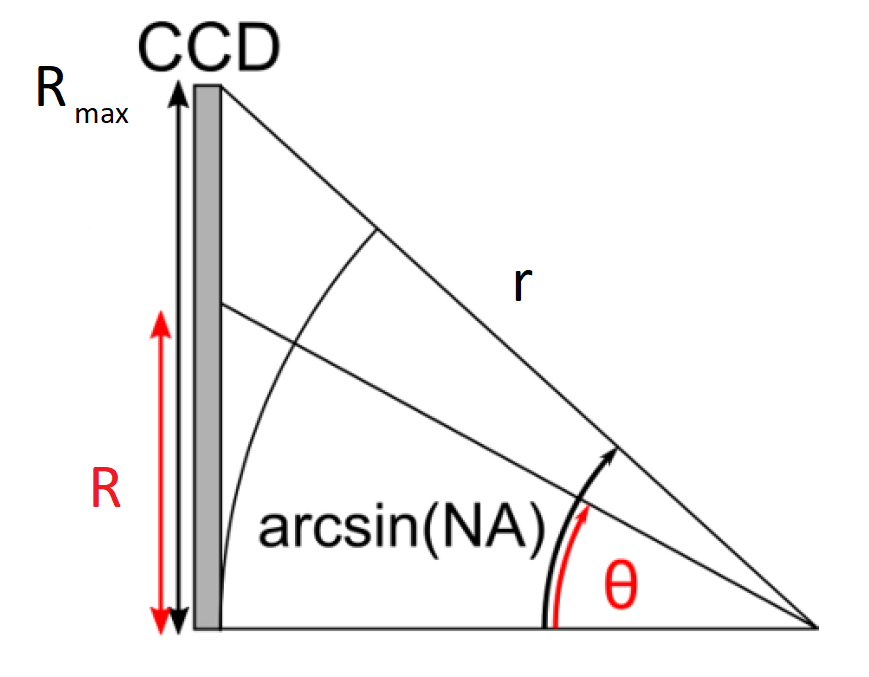
\includegraphics[width=0.3\textwidth]{Bilder/Anhang/arcsin}
\caption[Fourier-Korrektur]{Abbildung der Kugelwelle auf den CCD Schirm.}
\end{figure} Entsprechend der Abbildung ergibt sich \begin{equation}
sin(\theta)=\frac{R}{r} \Longleftrightarrow \theta =
arcsin\left(\frac{R}{r}\right) \text{ ,} \label{Korr1} \end{equation} gleichsam
gilt über die Definition der numerischen Apertur \begin{equation} NA=n(\lambda)
\, sin(\theta_{max}) \text{ ,} \end{equation} mit der optischen Dichte
n($\uplambda$) zwischen Objektiv und Probe. Es gilt also \begin{equation}
\frac{NA}{n(\lambda)}=\frac{R_{max}}{r} \Longleftrightarrow
r=\frac{n(\lambda)}{NA} \cdot R_{max} \text{ ,} \end{equation} für den
größtmöglichen Abstand der Abbildung zum Mittelpunkt des Detektors
R$_\text{max}$. Setzt man dieses nun in \autoref{Korr1} ein, so ergibt sich
\begin{equation} \theta=arcsin\left(\frac{NA}{n(\lambda)}\,
\frac{R}{R_{max}}\right)\text{ .} \label{Korr4} \end{equation} Die Überführung
der Messung am Detektor in den Raumwinkel skaliert also mit dem Arkussinus. Im
Folgenden werden $\frac{\text{NA}}{\text{n}(\uplambda)}=\text{a}$ und
$\frac{\text{R}}{\text{R}_\text{max}}=\text{z}$ gesetzt, sodass gilt
\begin{equation} \theta=arcsin\left(az\right) \text{ .} \end{equation} Möchte
man nun die Intensitäten korrigieren, so wird schnell ersichtlich, dass sich die
Fläche der Bestrahlung vergrößert, die Intensitäten für höhere Raumwinkel also
vermindert sind. Geht man davon aus, dass die gesamte Strahlung auf den Detektor
fällt, so bleibt die Gesamtintensität erhalten und zwar in allen
Koordinatensystemen. Es muss gelten: \begin{equation} I_{ges}=\int
\limits_{\Omega^{\ast}} \! \mathrm{d}x \, \mathrm{d}y \,\, \frac{I}{A}(x,y) =
\int \limits_\Omega \! \mathrm{d}\theta \, \mathrm{d}\varphi \,\, K(\theta)
\cdot \frac{I}{A}(\theta, \varphi) \text{ ,} \end{equation} mit einem
Korrekturfaktor K($\uptheta$).\\ Der Korrekturfaktor folgt der
Koordinatentransformation und ergibt sich zur Jacobi-Determinante
\begin{equation} K(\theta)&= \mathrm{det} \left(\begin{matrix} \frac{\partial
x}{\partial \theta} & \frac{\partial x}{\partial \varphi} \\ \frac{\partial
y}{\partial \theta} & \frac{\partial y}{\partial \varphi} \end{matrix}
\right)=r^2 \cdot sin(\theta) \cdot cos(\theta)\\ \text{mit } x&= r \cdot
cos(\theta) \cdot cos(\varphi) \notag\\ y&= r \cdot cos(\theta) \cdot
sin(\varphi) \notag \text{ ,} \end{equation} daraus folgt \begin{equation}
I_{ges}=\int \limits_{\Omega^{\ast}} \! \mathrm{d}x \, \mathrm{d}y \,\,
\frac{I}{A}(x,y) = \int \limits_\Omega \! \mathrm{d}\theta \, \mathrm{d}\varphi
\,\, r^2 \cdot sin(\theta) \cdot cos(\theta)\, \frac{I}{A}(\theta, \varphi)
\text{ ,} \end{equation} mit der Definition des Raumwinkels als \begin{equation}
\mathrm{d}\omega= r \, \mathrm{d}\theta \,\,\, r \,sin(\theta)
\,\mathrm{d}\varphi \end{equation} ergibt sich das Integral zu \begin{equation}
I_{ges}=\int \limits_{\Omega^{\ast}} \! \mathrm{d}x \, \mathrm{d}y \,\,
\frac{I}{A}(x,y) = \int \limits_\Omega \! \mathrm{d}\omega \, cos(\omega) \,\,
\frac{I}{A}(\omega) \text{ ,} \end{equation} mit dem Korrekturfaktor
\begin{equation} K(\omega)=cos (\omega) \text{ .} \end{equation} Jeder Pixel auf
der CCD integriert nun die lokale Intensitätsdichte über seine infinitesimal
kleine Fläche und fixiert somit örtlich einen Intensitätswert. \begin{equation}
I_{ges}= \sum_N \int \limits_{Pixel(x,y) } \! \mathrm{d}x \, \mathrm{d}y \,\,
\frac{I}{A}(x,y) = \sum_N \int \limits_{Pixel(\omega)} \! \mathrm{d}\omega \,
cos(\omega) \, \frac{I}{A}(\omega) \end{equation} Alle Pixel im Raumwinkelsystem
sind gleich groß. Für eine kleine Ausdehnung der Pixel im Raumwinkelsystem
gegenüber der Krümmung der Raumwinkelkugel lassen sie sich als annähernd planar
beschreiben. Für jeden einzelnen Pixel N mittelt sich also der Raumwinkel zu
\begin{equation} \overline{\omega} = \frac{\omega_{begin} + \upomega_{end}}{2}
\text{ .} \end{equation} Damit lässt sich das Integral zu \begin{equation}
\sum_N \int \limits_{Pixel(x,y)} \! \mathrm{d}\omega \,\, cos(\overline{\omega})
\, \frac{I}{A}(\omega) = \sum_N  cos(\overline{\omega})  \cdot \int
\limits_{Pixel(\omega)} \! \mathrm{d}\omega  \, \frac{I}{A}(\omega) \text{ .}
\end{equation} vereinfachen, da der Faktor $cos(\overline{\omega})$ vom Integral
unabhängig wird und somit vorgezogen werden kann. Löst man nun beide Integrale,
ergeben sich die aufintegrierten Intensitätsdichten der Pixel der jeweiligen
Systeme. Es gilt also die Gleichung \begin{equation} \sum_N I_{Pixel}(x,y) =
\sum_N cos(\overline{\omega}) \, I_{Pixel}(\overline{\omega})  \text{ ,}
\end{equation} mit der sich die Intensitäten der Pixel der jeweiligen Systeme
ineinander transformieren lassen. Für den einzelnen Pixel gilt also die
Gleichung \begin{equation} I_{Pixel}(\overline{\omega}) =
\frac{1}{cos(\overline{\omega})} \, I_{Pixel}(x,y) \text{ ,} \label{Korr2}
\end{equation} die die Pixeln der CCD-Kamera in die der Raumwinkelpixel
transformiert.\\ \\ Vereinfacht gesprochen muss also Folgendes berücksichtigt
werden:\\ Denken wir uns in ein Bild in dem ein Strahl der \textbf{Breite$=$1
Pixel} und der \textbf{Intensität$=$1} gerade also im
$\upomega=\textbf{0$^\circ$}$ \textbf{Winkel} auf die CCD-Kamera fällt. Der
Strahl hat nun die Intensitätsdichte$=$1.\\ Der selbe Strahl trifft nun im
$\upomega=\textbf{60$^\circ$}$ \textbf{Winkel} auf die CCD, er trifft  auf genau
\textbf{zwei Pixel}. Jeder Pixel sieht also die \textbf{Intensität$=1/2$}. Jeder
Pixel stellt mathematisch einen Punkt dar. Der Abstand dieser Punkte ist gegeben
durch den Abstand der Mittelpunkte ihrer Pixel. Für höhere Raumwinkel müssen
also mehrere Pixel zu einem einzigen zusammengefasst werden. Dazu werde die
Abstände der mathematischen Punkte mit dem Korrekturfaktor
K($\upomega$)=cos($\upomega$) verringert. Für die graphische Darstellung hat
sich jetzt aber nur künstlich die Pixeldichte erhöht und auch wenn sich im
mathematischen Sinne nun die Intensitätsdichte$=$ 2 x (Intensität$=1/2$) für die
Raumwinkel korrigiert hat, bleibt die dargestellte Intensität der Einzelpixel
unverändert zu gering, da die Pixel nicht aufsummiert werden, sondern jeder für
sich stehen bleibt. Es reicht also nicht aus, die Abstände zu verändern, sondern
jeder einzelne Punktintensität muss für die Darstellung korrigiert werden. Mit
der \autoref{Korr4} ergibt sich außerdem \begin{equation} I(\omega)=
\frac{1}{\sqrt{1-a^2z^2}} \, I(R) \label{Korr3} \end{equation} Folglich ergeben
sich zwei Möglichkeiten die Messung anzupassen. Entweder vor der Skalierung in
die Raumwinkel über die Abstände R der Pixel zum Zentrum und der Korrektur
\autoref{Korr3} oder nach der Skalierung in die Raumwinkel über den Winkel
$\upomega$ nach der Korrektur \autoref{Korr2}. \newpage \section{Einmessung der
Fourieroptik} \label{fourier} Nachdem die $\upmu$-PL fertig einjustiert wurde,
kann begonnen werden, die Fourier- und die Abbildungslinse \textbf{L2} und
\textbf{L4} einzumessen. \begin{itemize} \item Target \textbf{T4} in Filterwheel
und \textbf{T3} in Objektivhalter einsetzen, Hilfsspiegel M7 einsetzen, Beamwalk
nach obiger Anleitung \item Abbildungslinse \textbf{L4} ausbauen, Schraubtarget
\textbf{T6} einsetzen, mit Spiegel \textbf{M9} Strahl mittig aufs \textbf{T6}
zentrieren \item Fourierlinse \textbf{L2} in den Strahlengang klappen, Linse
entfernen und Schraubtarget \textbf{T7} einsetzen, mit den Stellschrauben  das
Target in den Laserstrahl zentrieren \item Schraubtarget \textbf{T6} entfernen
und Linse einsetzen \item Fourierlinse verdrehen, um auf Target \textbf{T6} zu
zentrieren \item Danach erneut Target \textbf{T7} einsetzen und erneut im
Laserstrahl mittels Stellschrauben zentrieren, Target \textbf{T7} entfernen und
\textbf{T8} in \textbf{L4} einsetzen \item Mit den Stellschauben mittig in den
Laser zentrieren, danach Target entfernen und Linse \textbf{L4} einsetzen \item
Verdrehen, bis mittig, dann erneut Target einsetzen und zentrieren \item Shutter
schließen, Abbildungs- und Fourierlinse einsetzen, Hilfsspiegel \textbf{M7}
entfernen \item  Mithilfe eines Spiegels hinter Pinhole \textbf{P3} Strahl aus
dem üblichen Strahlengang auskoppeln und mithilfe eines zweiten Spiegels hinter
dem Cage führen und mithilfe eines dritten Spiegels auf Target \textbf{T3}
zentrieren, der Strahlengang muss nicht dem Beamwalk genügen. \item \textbf{OD1}
Filter auf ``Blank'' stellen, Objektiv einsetzen, um Fourierlinse mithilfe von
Bodenplatten Führungsschiene bauen, Filter auf 4 Größenordnungen stellen \item
Mithilfe der CCD und dem Focusmodus der Software bei 5000 $\upmu$m Slitweite
Fourierbild des Laserstrahls bei kurzer Belichtungszeit darstellen \item Da
Laserstrahl paralleles Licht, bildet Fourierlinse den Strahl in einem Punkt ab,
durch Variation des Abstandes der Linse \textbf{L2} zum Objektiv komplette
Intensität auf möglichst wenige Pixel konzentrieren. Wenn erfolgt, für Linse
\textbf{L4} wiederholen. \end{itemize} \newpage \section{Fehlerabschätzung und
Hintergrundrauschen} \label{Fehler} Um die Aussagekraft der ermittelten
Messwerte einordnen zu können, sollen im Folgenden mögliche Abweichungen und die
daraus resultierenden Fehler berechnet werden. Sämtliche hier aufgeführte
Formeln wurden in das Matlab-Auswertungskript implementiert und für jede Messung
automatisiert berechnet. Es sollen im Folgenden die maßgeblichen Fehler
betrachtet werden. \subsection{Fehler der Fourierkoeffizienten}
\subsubsection{Schwankung der PL-Emission} Die PL-Emission der Nanodrähte
korreliert eng mit der Anregungsleistung des verwendeten Nd:YAG-Lasers. Diese
unterliegt jedoch gewissen Schwankungen, die berücksichtigt werden müssen und
sich direkt auf die Emission auswirken. Um die Effekte möglichst linear
beschreiben zu können, muss der Nanodraht deutlich im Lasingbereich angeregt
werden, da es ansonsten schnell durch die superlineare Steigung im Bereich der
ASE zu hohen Fehlern kommen kann. Die mittlere Anregungsdichte p des Lasers wird
mithilfe der Messdiode bestimmt und mit einer Standardabweichung s$_\text{p}$
ausgegeben. Es wurden jeweils N$=$500 Messintervalle à 0.2 s gemittelt. Für ein
Vertrauensniveau von 2$\sigma$ ergibt sich mit $\uptau=\text{1.965}$ der Fehler
zu \begin{equation} \Delta p = \frac{s_p}{\sqrt{N}} \cdot \tau \text{ .}
\end{equation} Dieser Fehler wiederum setzt sich in der PL-Intensität fort.
Anhand der Casperson-Anpassung, die die Anregungsdichte mit der PL-Intensität
des Nanodrahtes in Beziehung setzt, kann dieser Fehler ermittelt werden.\\ Es
gilt: \begin{equation} \Delta I_{PL}= I_{PL}(p+ \Delta p)-I_{PL}(p) \qquad
\text{bzw.} \qquad \frac{\Delta I_{PL}}{p}= \frac{I_{PL}(p + \Delta
p)-I_{PL}(p)}{I_{PL}} \text{ .} \end{equation} Für den Intensitätsfehler eines
jeden Bildes gilt also: \begin{equation} \Delta I_{n} = \frac{\Delta
I_{PL}}{I_{PL}}\, \cdot \, I_{n} \text{ .} \end{equation} Damit folgt der Fehler
der Fourierkoeffizienten aus \autoref{FourKoeff}: \begin{equation} \Delta
A_I&=\frac{2}{N} \, \sum_{n=1}^N \left| I_n \cdot \left( \frac{\Delta
I_{n}}{I_{n}}\right)\right| \text{ ,} \,\quad\qquad\qquad\, \Delta
B_I=\frac{4}{N} \, \sum_{n=1}^N \left| I_n \, sin(2\theta) \cdot \left(
\frac{\Delta I_{n}}{I_{n}}\right) \right| \text{ ,} \notag \\ \Delta
C_I&=\frac{4}{N} \, \sum_{n=1}^N \left| I_n \, cos(4\theta) \cdot \left(
\frac{\Delta I_{n}}{I_{n}}\right)\right| \text{ ,} \qquad \Delta D_I=\frac{4}{N}
\, \sum_{n=1}^N \left| I_n \, sin(4\theta) \cdot \left( \frac{\Delta
I_{n}}{I_{n}}\right)\right| \text{ .} \label{FehlerI} \end{equation}
\subsubsection{Genauigkeit der Rotation} Zur Berechnung der Fourierkoeffizienten
muss die $\uplambda$/4-Platte rotiert werden. Die Einstellung der richtigen
Winkel ist also auf den Ablesefehler begrenzt. Dieser soll als ein Viertel
Skalenteil resp. $\Updelta \uptheta =\text{0.5}^\circ$ angenommen werden. Nach
\begin{equation} &\Delta A_\theta= \frac{\partial A}{\partial \theta} \cdot
\Delta \theta \qquad\qquad\text{ ,} \Delta B_\theta= \frac{\partial B}{\partial
\theta}\cdot \Delta \theta\text{ ,} \notag \\ &\Delta C_\theta= \frac{\partial
C}{\partial \theta}\cdot \Delta \theta\text{ ,} \qquad\qquad \Delta D_\theta=
\frac{\partial D}{\partial \theta}\cdot \Delta \theta\text{ ,} \end{equation}
und \autoref{FourKoeff} ergibt sich für den Fehler der Fourierkoeffizienten
\begin{equation} &\Delta A_\theta= 0 \text{ ,}
\qquad\qquad\qquad\qquad\qquad\qquad\quad\,\,\, \Delta B_\theta = \frac{4}{N} \,
\sum_{n=1}^N \left| 2\, I_n \, cos(2\,\theta)\cdot \frac{\pi}{180^\circ} \,
\Delta\theta \right| \text{ ,} \notag \\ &\Delta C_\theta=\frac{4}{N} \,
\sum_{n=1}^N \left| 4\, I_n \, sin(4\,\theta)\cdot \frac{\pi}{180^\circ} \,
\Delta\theta\right| \text{ ,} \quad\, \Delta D_\theta=\frac{4}{N} \,
\sum_{n=1}^N \left| 4\, I_n \, cos(4\,\theta)\cdot \frac{\pi}{180^\circ} \,
\Delta\theta\right| \text{ .} \label{FehlerTheta} \end{equation}\\
Zusammengefasst folgt aus \autoref{FehlerI} und \autoref{FehlerTheta} der
Gesamtfehler nach: \begin{equation} &\Delta A_{ges}= \Delta A_I \text{ ,}
\qquad\qquad\quad\, \Delta B_{ges}= \Delta B_I + \Delta B_\theta \text{
,}\notag\\ &\Delta C_{ges}= \Delta C_I + \Delta C_\theta \text{ ,} \qquad \Delta
D_{ges}= \Delta D_I + \Delta D_\theta \text{ .} \end{equation}
\subsection{Ausrichtung der optischen Elemente und Phasenverschiebung} Bei der
Ausrichtung der Transmissionsachse des Polarisators sowie der schnellen
optischen Achse der $\uplambda$/4-Platte kommt es zu kleinen Abweichungen
gegenüber dem gewünschten Koordinatensystem. Daraus resultieren kleine
Verschiebungen der Stokes-Paramter untereinander. Für den Winkel $\upalpha$ der
$\uplambda$/4-Platte $\upalpha$ wurde ein Fehler von $\Updelta
\upalpha=\text{1.2}^\circ$, für den Winkel des Polarisators ein Fehler von
$\Updelta \upbeta=\text{1.8}^\circ$ ermittelt (s. \autoref{AusrOptEl}). Die
Phasenverschiebung der $\uplambda$/4-Platte hängt stark vom Einfallswinkel des
Lichtes zur Flächennormale der $\uplambda$/4-Platte ab. Der Fehler soll mit
$\Updelta\updelta=3^\circ$ abgeschätzt sein. Durch die Position der
Transmissionsachse wird ein Koordinatensystem für die Stokes-Parameter
aufgespannt. Dieses System soll nun in das Koodinatensystem des Nanodrahtes
transformiert werden, sodass die vertikale y-Achse der c-Achse des Nanodrahtes
entspricht. Der Winkel zwischen Transmissionsachse und c-Achse des Nanodrahtes
$\upbeta$ ist gegeben durch die Differenz beider Winkel $\Updelta \upbeta$
zwischen Transmissionsachse des Polarisators und Laborsystem sowie
Nanodrahtachse und Laborsystem. Der Fehler des Winkels des Nanodrahts soll mit
$\Updelta \upbeta_\text{NW}=\text{0.5}^\circ$ abgeschätzt werden. Somit wird der
Gesamtfehler der Ausrichtung des Polarisators als $\Updelta
\upbeta_{ges}=\text{2.3}^\circ$ angenommen.\\ Aus den \autoref{StokesGL5} folgen
für die Stokes-Parameter die Fehlerfortpflanzungen:\\\\ \underline{für den
S$_\text{0}$-Parameter} \begin{equation} \Delta S_0=& \Delta A_{ges} +
\frac{1+cos(\delta)}{1-cos(\delta)} \Delta C_{ges} + \frac{\partial
S_0}{\partial \delta} \cdot \Delta \delta \notag\\ =&\Delta A_{ges} +
\frac{1+cos(\delta)}{1-cos(\delta)} \, \Delta C_{ges} + 2\,
\frac{sin(\delta)}{(1-cos(\delta))^2}\, \frac{\pi}{180^\circ}\, C \cdot \Delta
\delta \end{equation}\\ \underline{für den S$_\text{1}$-Parameter}
\begin{equation} \Delta S_1= \frac{2}{1-cos(\delta)}\,\left[ \Delta C_{ges}\cdot
cos(2\,\beta) + \Delta D_{ges}\cdot sin(2\beta)\right] + \frac{\partial
S_1}{\partial \delta} \cdot \Delta \delta + \frac{\partial S_1}{\partial
\beta}\cdot \Delta \beta \notag \end{equation} \begin{multline} \Delta S_1=
\frac{2}{1-cos(\delta)}\,\left[ \left( \Delta
C_{ges}+\frac{\pi}{180^\circ}\,\Delta \delta \,
\frac{sin(\delta)}{1-cos(\delta)} \, C \right) \cdot cos(2\,\beta) \right]\\ +
\frac{2}{1-cos(\delta)}\,\left[ \left( \Delta
D_{ges}+\frac{\pi}{180^\circ}\,\Delta \delta \,
\frac{sin(\delta)}{1-cos(\delta)} \, D \right) \cdot cos(2\,\beta) \right]+
\frac{\partial S_1}{\partial \beta}\cdot \Delta \beta \notag \end{multline}
\begin{multline} \Delta S_1= \frac{2}{1-cos(\delta)}\,\left[ \left( \Delta
C_{ges}+\frac{\pi}{180^\circ}\,\left( \Delta \delta \,
\frac{sin(\delta)}{1-cos(\delta)} \, C + 2\,D \cdot \Delta\beta\right) \right)
\cdot cos(2\,\beta) \right]\\ \qquad\,\,\, + \frac{2}{1-cos(\delta)}\,\left[
\left( \Delta D_{ges}+\frac{\pi}{180^\circ}\,\left( \Delta \delta \,
\frac{sin(\delta)}{1-sin(\delta)} \, D -2\, C \cdot \Delta\beta\right)\right)
\cdot sin(2\,\beta) \right] \end{multline} \underline{für den
S$_\text{2}$-Parameter} \begin{multline} \Delta S_2=
\frac{2}{1-cos(\delta)}\,\left[ \left( \Delta
D_{ges}+\frac{\pi}{180^\circ}\,\left( \Delta \delta \,
\frac{sin(\delta)}{1-cos(\delta)} \, D + 2\,C \cdot \Delta\beta\right) \right)
\cdot cos(2\,\beta) \right]\\ \qquad\,\,\,\, + \frac{2}{1-cos(\delta)}\,\left[
\left( \Delta C_{ges}+\frac{\pi}{180^\circ}\,\left( \Delta \delta \,
\frac{sin(\delta)}{1-cos(\delta)} \, C -2\, D \cdot\Delta\beta\right)\right)
\cdot sin(2\,\beta) \right] \end{multline} \underline{für den
S$_\text{3}$-Parameter} \begin{equation} \Delta S_3&= \frac{2}{sin(x)}\left
[\Delta B_{ges} + 2\, \frac{1}{tan(\delta)} \frac{\pi}{180^\circ}\, \Delta
\delta\cdot B\right] \end{equation} \underline{für die lineare Polarisation}
\begin{equation} \Delta P_{Lin}&= \frac{2}{1-cos(\delta)}\, \left[
\frac{sin(\delta)}{1-cos(\delta)} \, \sqrt{C^2+D^2} \, \frac{\pi}{180^\circ} \,
\Delta \delta + \frac{\Delta C\cdot C + \Delta D \cdot D}{\sqrt{C^2+D^2}}
\right]\notag\\ &=\frac{1}{1-cos(\delta)}\, \left[ sin(\delta)\,
\sqrt{S_1^2+S_2^2} \, \frac{\pi}{180^\circ} \, \Delta \delta + 2\, \frac{\Delta
C\cdot C + \Delta D \cdot D}{\sqrt{C^2+D^2}}  \right] \end{equation}
\underline{für die Gesamtpolarisation} \begin{multline} \Delta P_{ges}=
\frac{\left[ \left( \frac{4\,sin(\delta)}{(1-cos(\delta))^3}(C^2+D^2) +
\frac{1}{tan(\delta)\, sin^2(\delta)}\, B^2
\right)\frac{\pi}{180^\circ}\,\Delta\delta\right]}{\sqrt{S_1^2+S_2^2+S_3^3}}\\ +
\frac{\left[ \frac{4}{(1-cos(\delta))^2}\, (\Delta C\cdot C + \Delta D \cdot D)
+ \frac{1}{sin^2(\delta)}\,\Delta B \cdot B)
\right]}{\sqrt{S_1^2+S_2^2+S_3^3}}\notag \end{multline} \begin{multline} \Delta
P_{ges}= \frac{\left[ \left( \frac{sin(\delta)}{1-cos(\delta)}(S_1^2+S_2^2) +
\frac{1}{tan(\delta)}\, S_3^2
\right)\frac{\pi}{180^\circ}\,\Delta\delta\right]}{\sqrt{S_1^2+S_2^2+S_3^3}}\\ +
\frac{\left[ \frac{4}{(1-cos(\delta))^2}\, (\Delta C\cdot C + \Delta D \cdot D)
+ \frac{1}{sin^2(\delta)}\,\Delta B \cdot B \right]}{\sqrt{S_1^2+S_2^2+S_3^3}}
\end{multline} \underline{für den horizontalen Feldanteil} \begin{equation}
\Delta \langle E_x \rangle^2 =\frac{1}{2}\, \left[ \Delta A_{ges} + \Delta
C_{ges} \right] \end{equation} \underline{für den vertikalen Feldanteil}
\begin{equation} \Delta \langle E_y \rangle^2 =\frac{1}{2}\, \left[ \Delta
A_{ges} + \frac{3+cos(\delta)}{(1-cos(\delta))^2} \cdot \Delta C_{ges}
+\frac{4\, sin(\delta)}{(1-cos(\delta))^2} \, \frac{\pi}{180^\circ} \, C \cdot
\Delta\delta \right] \end{equation} Für den Fehler der Ausrichtung der
$\uplambda$/4-Platte bedeutet diese Transformation eine zusätzliche Addition des
Fehlers der Ausrichtung des Polarisators auf den ursprünglichen Fehler. So
ergibt sich $\Updelta \upalpha_{ges} = \text{1.8} + \text{1.2} =\text{3}^\circ$.
Der Fehler für die Unsicherheit des Winkels $\uptheta$ ergänzt sich also um die
Terme: \begin{equation} &\Delta A_\theta= 0 \text{ ,} \\ &\Delta B_\theta =
\frac{4}{N} \, \sum_{n=1}^N  2\, I_n \, cos(2\,\theta)\cdot
\frac{\pi}{180^\circ} \, \Delta \alpha_{ges}  \text{ ,}\\ &\Delta
C_\theta=\frac{4}{N} \, \sum_{n=1}^N  4\, I_n \, sin(4\,\theta)\cdot
\frac{\pi}{180^\circ} \, \Delta \alpha_{ges} \text{ ,}\\ &\Delta
D_\theta=\frac{4}{N} \, \sum_{n=1}^N  4\, I_n \, cos(4\,\theta)\cdot
\frac{\pi}{180^\circ} \,  \Delta \alpha_{ges} \text{ .} \end{equation} Die
Fehler der Ausrichtung der $\uplambda$/4-Platte $\Updelta \upalpha$ und der
Transmissionsachse des Polarisators $\Updelta \upbeta$ sowie der Fehler der
Verschiebung der $\uplambda$/4-Platte sind systematischer Natur. Für die
vergleichenden Messungen mit angelegten Magnetfeldern ändern sie sich nicht. Sie
führen zu den jeweils gleichen Abweichungen und können für den Vergleich
ausgeblendet werden. \subsection{Kosmische Strahlung und Hintergrundrauschen}
\label{Rauschen} Gleichzeitig lässt sich über die Vielzahl der aufgenommenen
Hintergründe gleicher Messmethode in dieser Masterthesis eine Varianz der
gemessenen Hintegrundintensität jedes Pixels ermitteln. Das Rauschen beträgt im
Mittel $\Updelta= \text{0.2}$ Counts/s. Unterhalb dieser Grenze ist eine
Änderung nicht signifikant.\\ Um zu verhindern, dass durch Rauschen oder
kosmische Strahlen das Ergebnis verzerrt wurde, werden Pixel mit einem
Polarisationsgrad DOP $\geq$ 2 aus den Bildern entfernt, sie erscheinen weiß.
\section{Ergänzungen zur Berechnung der Stokes-Parameter} \label{StokesFalsch}
In der Literatur finden sich vereinzelt Berechnungen $\text{B} \sim
\sum_{\text{n}=\text{1}}^\text{N} \text{I}_\text{n} \,
\text{sin}(\text{2}\uptheta)$ \cite{Berry.1977,Anleitung}, von solch einer
Berechnungen wird in dieser Masterthesis Abstand genommen:\\ Für gesamtheitlich
linkszirkular polarisiertes Licht ($\text{S}_\text{0}=\text{1}$,
$\text{S}_\text{3}=\text{-1})$ ergibt sich nach \autoref{StokesGleichung} die
Gesamtintensität zu \begin{equation} I(\theta)= \frac{1}{2}\left[ S_0 + S_3 \,
sin(2\, \theta)\right]=\frac{1}{2} \, (1 - sin(2 \, \theta)) \text{ .}
\end{equation} Eine Faltung nach \cite{Goldstein.2003} mit einem Kosinus- statt
Sinusterm zur Berechnung des Fourierkoeffizienten B führt zum Widerspruch, nur
mit dem Sinus ist folglich die korrekte Berechnung des S$_\text{3}$-Parameters
möglich. \begin{equation} S_3^\ast &=B^\ast= \frac{2}{\pi} \int_0^{2\,\pi} \,
d\theta \, I(\theta) \, cos(2\, \theta)= \frac{1}{\pi} \int_0^{2\,\pi} \,
d\theta (1 - sin(2\, \theta)) \, cos(2\, \theta)=0 \\ S_3&=B= \frac{2}{\pi}
\int_0^{2\,\pi} \, d\theta \, I(\theta) \, sin(2\, \theta)= \frac{1}{\pi}
\int_0^{2\,\pi} \, d\theta (1 - sin(2\, \theta)) \, sin(2\, \theta)=-1
\end{equation} \section{Spin Injektion} \label{Spininjection} Die
Überbevölkerung eines Spinzustandes durch externe Einflüsse wird als
\textit{Spin Injektion} bezeichnet und kann über verschiedene Wege erreicht
werden. Zunächst ist es möglich, einen ausgewählten Bandübergang durch
polarisiertes Licht zu begünstigen. Beschränkt man sich energetisch auf die HH-
und LH-Bänder, so wäre mit zirkulär polarisiertem Licht eine Polarisation
$\text{P}=\frac{\text{3}-\text{1}}{\text{3}+\text{1}}=\text{50}\%$
($P_\text{spin}=\text{2} \cdot \text{P}_\text{circ}$) zu erwarten. Durch die
geringe Aufspaltung beider Bänder kommt es jedoch zu einem Überlapp beider
strahlenden Übergänge, so dass Elektronen beider Bänder angeregt und, daraus
resultierend, beide Polarisationszustände gleichzeitig besetzt werden. Für die
maximale Polarisation gilt hier: \begin{equation}
&a^2=\frac{\alpha_B}{\alpha_A}\\ &a=\frac{1}{x \cdot \sqrt{\frac{1}{x^2}+1}}
&x=\frac{-(\Delta_1-\Delta_2)+\sqrt{(\Delta_1-\Delta_2)^2+8\cdot(\Delta_3)^2}}{2
\sqrt{2}\cdot \Delta_3} \end{equation} mit den Anregungswahrscheinlichkeiten der
Valenzbänder A und B $\upalpha_\text{A,B}$, dem Kristall-Feld Parameter für ZnO
$\Updelta_{\text{1}}=\text{43 meV}$ sowie der parallelen und orthogonalen
Spin-Bahn-Parameter bezüglich der c-Achse
$\Updelta_{\text{2}}=\Updelta_{\text{3}}=\Updelta_{\text{SO}}/3=\text{5.3 meV}$
\cite{Reynolds.1999} ergibt sich eine maximale Polarisation
$\text{P}_{\text{max}}=\text{1.5}\%$. Somit ist eine optische Polarisation für
unser Materialsystem quasi ausgeschlossen \cite[S. 299]{Morkoc.2009}, da auch
eine lineare Polarisation des Lichtes beide Spinzustände gleichermaßen
bevölkert.\\ \\ Magnetfelder bieten eine weitere Möglichkeit die Überpopulation
eines Spinzustandes herbeizuführen. Durch die Zeeman-Aufspaltung \ref{Zee} wird
die Entartung der beiden Spinzustände des Leitungsbandes aufgehoben.
Entsprechend stellt sich das thermische Gleichgewicht zugunsten des energetisch
abgesenkten Zustandes neu ein.\\ \\ Da elektrische Felder in dieser Thesis keine
Verwendung finden, wird eine elektrische Spin Injektion hier nicht betrachtet,
soll der Vollständigkeit halber aber erwähnt werden.
